\section{Results – Strategy S4: Multi-LLM Per-Field}
\label{sec:eval-s4}

The \textbf{S4: Multi-LLM Per-Field} strategy applies consensus at the slot level: each field is extracted by multiple models and consolidated via a field-aware verifier. We evaluate three variants: \textbf{S4.0} without few-shot prompting on the original MUC-4 dataset, \textbf{S4.1} with few-shot prompting on the original dataset, and \textbf{S4.2} with few-shot prompting on a speech-style variant.

Figure~\ref{fig:s4-variants-bar} shows that per-field consensus behaves differently from the other strategies: it produces strong nonempty-field performance (high NES) but tends to overfill slots, as reflected in the negative EAI values and elevated hallucination rates. This indicates that the model ensemble is biased toward producing a value rather than abstaining. Few-shot prompting moderates this behaviour slightly by reducing hallucinations and improving overall accuracy, though the conservative–vs.–aggressive fill trade-off persists. The speech-style variant remains close to the clean-text version, showing that slot-wise consensus dampens some noise effects but does not fully counteract the tendency to oversupply values.

Per-field consensus boosts \texttt{incidentLocation}; \texttt{perpetratorIndividual} remains hardest; \texttt{weapon} is lower than in S1 and S3.

Figure ~\ref{fig:s4-perfield-plot} illustrates the asymmetric effects of per-field voting on different slots. \texttt{incidentLocation} benefits most, reaching an average score of $0.641$ in S4.1 and surpassing the corresponding values in the single-pass and full-document consensus strategies, which suggests that slot-specific prompts plus ensemble agreement help to stabilise location predictions. \texttt{incidentStage} also performs strongly ($0.720$), consistent with its comparatively structured label space. In contrast, \texttt{incidentType} and especially \texttt{incidentDate} underperform relative to other strategies (down to $0.370$ for dates), which indicates that aggressive filling at the field level can lead to more spurious or partially incorrect outputs when the signal is weak. \texttt{weapon} achieves $0.692$, clearly lower than in S1 and S3, suggesting that per-field voting may over-accept marginal mentions and noise in this slot. \texttt{perpetratorIndividual} remains one of the hardest fields despite the richer consensus mechanism, reflecting the persistent difficulty of sparse, ambiguous references to individual actors.

\begin{figure}[H]
\centering
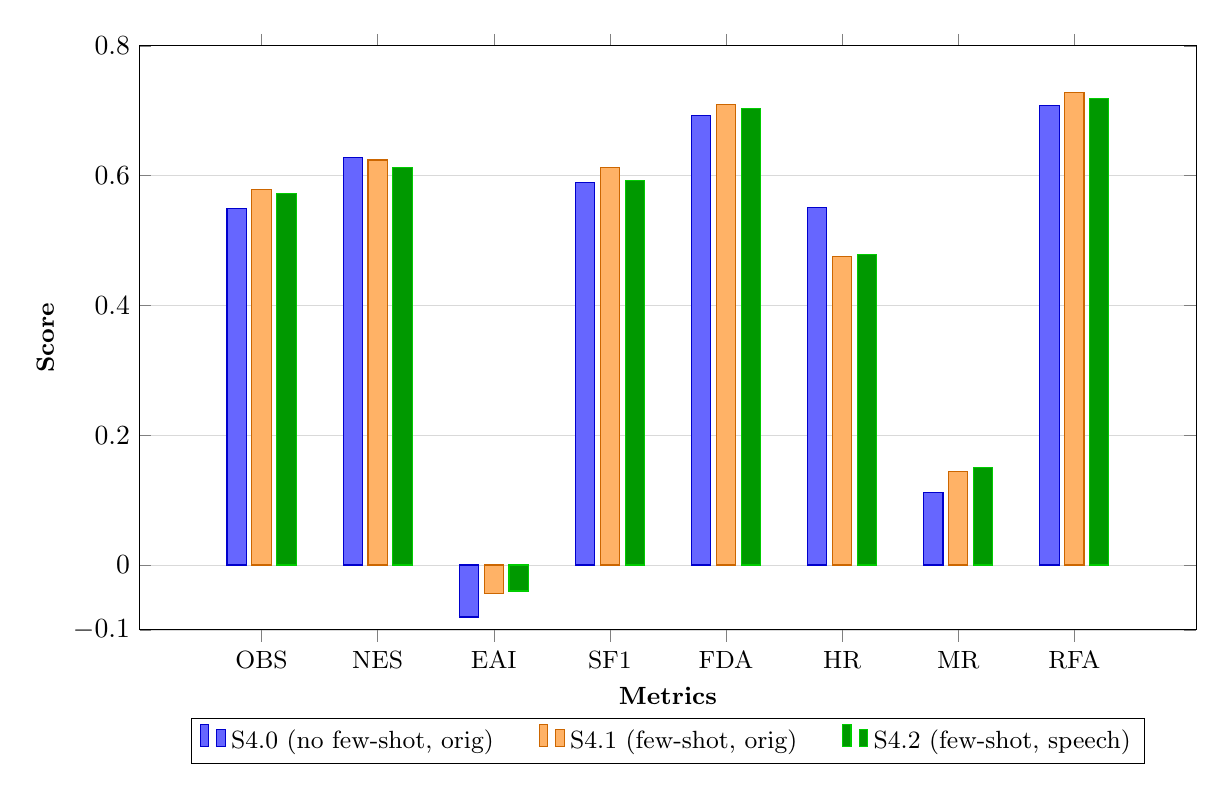
\begin{tikzpicture}
  \begin{axis}[
    width=15cm,
    height=9cm,
    ybar,
    bar width=7pt,
    ylabel={Score},
    ylabel style={font=\small\bfseries},
    xlabel={Metrics},
    xlabel style={font=\small\bfseries},
    symbolic x coords={OBS, NES, EAI, SF1, FDA, HR, MR, RFA},
    xtick=data,
    xticklabel style={font=\small},
    ymin=-0.1,
    ymax=0.8,
    ytick={-0.1, 0, 0.2, 0.4, 0.6, 0.8},
    ymajorgrids=true,
    grid style={line width=0.3pt, draw=gray!30},
    legend style={
      at={(0.5,-0.15)},
      anchor=north,
      legend columns=3,
      font=\small,
      /tikz/every even column/.append style={column sep=0.5cm}
    },
    enlarge x limits=0.15,
  ]
  
  % S4.0 (no few-shot, orig) - Blue
  \addplot[fill=blue!60, draw=blue!80!black] coordinates {
    (OBS, 0.549)
    (NES, 0.628)
    (EAI, -0.080)
    (SF1, 0.589)
    (FDA, 0.693)
    (HR, 0.551)
    (MR, 0.112)
    (RFA, 0.708)
  };
  \addlegendentry{S4.0 (no few-shot, orig)}
  
  % S4.1 (few-shot, orig) - Orange
  \addplot[fill=orange!60, draw=orange!80!black] coordinates {
    (OBS, 0.579)
    (NES, 0.624)
    (EAI, -0.044)
    (SF1, 0.613)
    (FDA, 0.709)
    (HR, 0.476)
    (MR, 0.144)
    (RFA, 0.728)
  };
  \addlegendentry{S4.1 (few-shot, orig)}
  
  % S4.2 (few-shot, speech) - Green
  \addplot[fill=green!60!black, draw=green!80!black] coordinates {
    (OBS, 0.572)
    (NES, 0.612)
    (EAI, -0.040)
    (SF1, 0.592)
    (FDA, 0.704)
    (HR, 0.479)
    (MR, 0.150)
    (RFA, 0.719)
  };
  \addlegendentry{S4.2 (few-shot, speech)}
  
  \end{axis}
\end{tikzpicture}
\caption{Headline metrics for S4 variants on MUC-4 ($N{=}100$). Few-shot prompting (S4.1) improves most accuracy-oriented metrics (OBS, SF1, FDA, RFA) but still produces negative EAI values, indicating disagreement across models at the slot level. The speech-style variant (S4.2) performs similarly to S4.1, suggesting that per-field consensus mitigates some ASR-related noise. Overall, S4 offers strong schema adherence but also highlights how per-field aggregation can amplify model inconsistencies.}
\label{fig:s4-variants-bar}
\end{figure}



\begin{figure}[H]
\centering
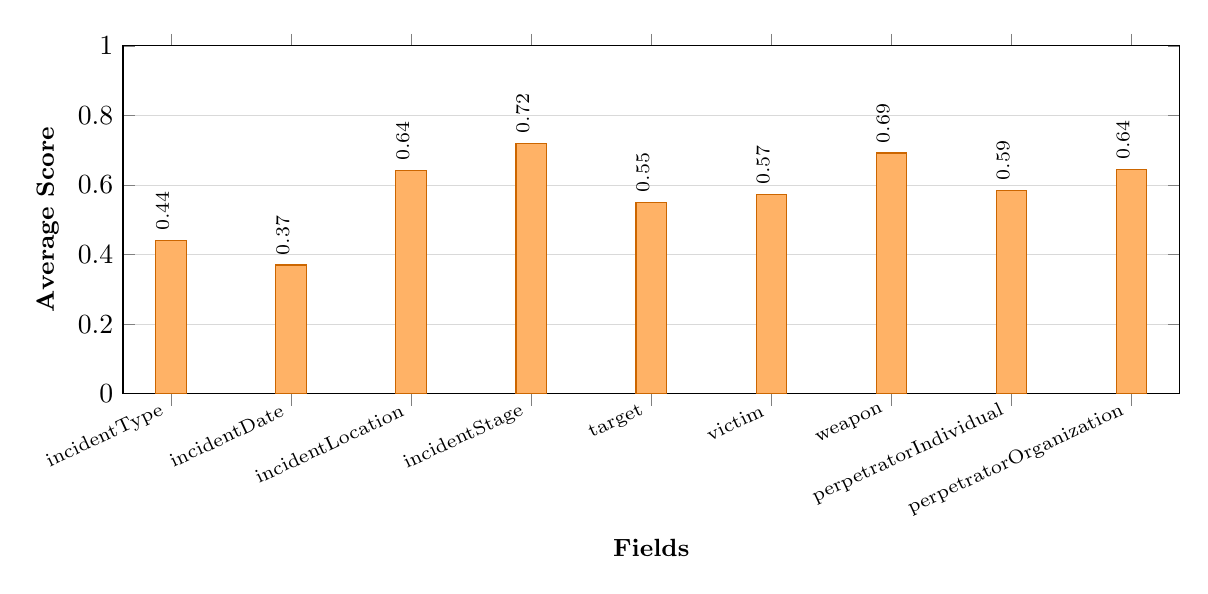
\begin{tikzpicture}
  \begin{axis}[
    width=15cm,
    height=6cm,
    ybar,
    bar width=11pt,
    ylabel={Average Score},
    ylabel style={font=\small\bfseries},
    xlabel={Fields},
    xlabel style={font=\small\bfseries},
    symbolic x coords={
      incidentType,
      incidentDate,
      incidentLocation,
      incidentStage,
      target,
      victim,
      weapon,
      perpetratorIndividual,
      perpetratorOrganization
    },
    xtick=data,
    xticklabel style={font=\scriptsize, rotate=25, anchor=east},
    ymin=0,
    ymax=1.0,
    ymajorgrids=true,
    grid style={line width=0.3pt, draw=gray!30},
    enlarge x limits=0.05,
    nodes near coords,
    nodes near coords style={
        font=\scriptsize,
        rotate=90,
        anchor=west,
        yshift=3pt
    }
  ]

  \addplot[fill=orange!60, draw=orange!80!black] coordinates {
    (incidentType, 0.440)
    (incidentDate, 0.370)
    (incidentLocation, 0.641)
    (incidentStage, 0.720)
    (target, 0.550)
    (victim, 0.572)
    (weapon, 0.692)
    (perpetratorIndividual, 0.585)
    (perpetratorOrganization, 0.644)
  };

  \end{axis}
\end{tikzpicture}
\caption{Per-field extraction performance for S4.1 on the MUC-4 subset ($N{=}100$). The per-field multi-LLM strategy performs well on structured fields such as \textit{incidentStage}, \textit{weapon}, and \textit{incidentLocation}, but struggles on more context-dependent fields like \textit{incidentType} and \textit{incidentDate}. This pattern shows how per-field consensus can stabilize well-defined slots while amplifying uncertainty in categories that require broader reasoning.}
\label{fig:s4-perfield-plot}
\end{figure}


\subsection*{Latency}

\begin{figure}[H]
\centering
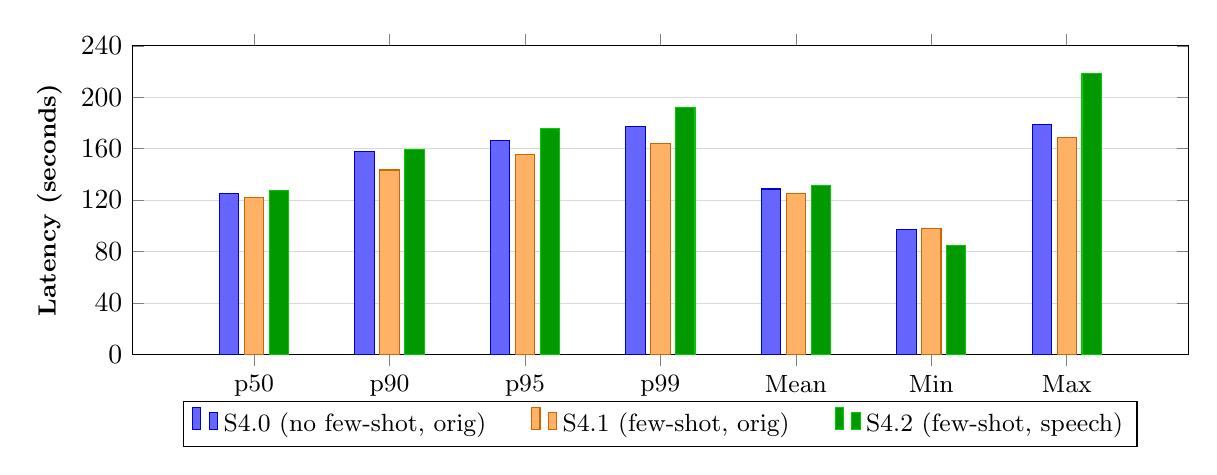
\begin{tikzpicture}
  \begin{axis}[
    width=15cm,
    height=5.5cm,
    ybar,
    bar width=7pt,
    ylabel={Latency (seconds)},
    ylabel style={font=\small\bfseries},
    xlabel={Statistics},
    xlabel style={font=\small\bfseries},
    symbolic x coords={p50, p90, p95, p99, Mean, Min, Max},
    xtick=data,
    xticklabel style={font=\small},
    ymin=0,
    ymax=240,
    ytick={0, 40, 80, 120, 160, 200, 240},
    ymajorgrids=true,
    grid style={line width=0.3pt, draw=gray!30},
    legend style={
      at={(0.5,-0.15)},
      anchor=north,
      legend columns=3,
      font=\small,
      /tikz/every even column/.append style={column sep=0.5cm}
    },
    enlarge x limits=0.15,
  ]
  
  % S4.0 (no few-shot, orig) - Blue
  \addplot[fill=blue!60, draw=blue!80!black] coordinates {
    (p50, 125.14)
    (p90, 157.96)
    (p95, 166.02)
    (p99, 177.27)
    (Mean, 128.64)
    (Min, 97.08)
    (Max, 179.00)
  };
  \addlegendentry{S4.0 (no few-shot, orig)}
  
  % S4.1 (few-shot, orig) - Orange
  \addplot[fill=orange!60, draw=orange!80!black] coordinates {
    (p50, 121.81)
    (p90, 143.39)
    (p95, 155.16)
    (p99, 164.08)
    (Mean, 124.98)
    (Min, 98.10)
    (Max, 168.81)
  };
  \addlegendentry{S4.1 (few-shot, orig)}
  
  % S4.2 (few-shot, speech) - Green
  \addplot[fill=green!60!black, draw=green!80!black] coordinates {
    (p50, 127.23)
    (p90, 159.02)
    (p95, 175.50)
    (p99, 192.16)
    (Mean, 131.15)
    (Min, 84.42)
    (Max, 218.22)
  };
  \addlegendentry{S4.2 (few-shot, speech)}
  
  \end{axis}
\end{tikzpicture}
\caption{Latency statistics for S4 variants (seconds). The per-field multi-LLM strategy shows the highest computational cost, with median latencies near 2 minutes and p99 values above 3 minutes. Few-shot prompting (S4.1) slightly lowers extreme latencies relative to S4.0, while the speech-style variant (S4.2) adds more variance. Overall, S4 highlights the trade-off between the robustness of per-field consensus and the considerable runtime required for multiple LLM calls.}
\label{fig:s4-latency-bar}
\end{figure}

Figure~\ref{fig:s4-latency-bar} makes clear that S4 is the slowest strategy family. All three variants have median latencies in the 122–127\,s range per document and heavy upper tails, with p99 values between roughly $164$\,s and $192$\,s. This behaviour is expected because S4 runs multiple models for each individual slot rather than once per document. Few-shot prompting slightly reduces median and mean latency when moving from S4.0 to S4.1, but the differences are small compared to the overall cost of per-field ensemble processing. S4.2 is marginally slower than S4.1 on average and exhibits the heaviest tail (Max above $218$\,s), reflecting additional variability in convergence on speech-style inputs. In comparison to S3.1, which also uses multi-LLM consensus but at the document level, S4 sacrifices throughput for more aggressive slot-level filling; this makes it less attractive for high-volume or time-sensitive deployments unless very high recall on nonempty fields is the primary objective.

\subsection*{Cost Analysis (S4: Multi-LLM Per-Field Consensus)}

\textbf{Assumptions.} For each of the $F{=}9$ fields, two parallel extractions are run—\textit{GPT-5} and \textit{Gemini~2.5~Pro}—with per-field averages $i_f{=}1{,}500$ input tokens and $o_f{=}50$ output tokens. A single arbiter/verification step per record runs on \textit{GPT-5-mini} with $V_{\text{in}}{=}1{,}000$ and $V_{\text{out}}{=}100$. If audio is used, Whisper transcription for $D$ minutes is added once per record.

\textbf{Prices.} GPT-5: input \$1.25/M, output \$10.00/M. Gemini~2.5~Pro: input \$1.25/M, output \$10.00/M. GPT-5-mini: input \$0.25/M, output \$2.00/M. Whisper: \$0.006/min.

\textbf{Formula.}
\[
\text{Cost}_{\text{S4}} =
\sum_{f=1}^{F}\!\Big[
\underbrace{\tfrac{i_f}{10^6}p_{\text{in}}^{(5)} + \tfrac{o_f}{10^6}p_{\text{out}}^{(5)}}_{\text{GPT-5 per field}}
+
\underbrace{\tfrac{i_f}{10^6}p_{\text{in}}^{(\text{Gemini})} + \tfrac{o_f}{10^6}p_{\text{out}}^{(\text{Gemini})}}_{\text{Gemini per field}}
\Big]
+\underbrace{\tfrac{V_{\text{in}}}{10^6}p_{\text{in}}^{(\text{mini})}+\tfrac{V_{\text{out}}}{10^6}p_{\text{out}}^{(\text{mini})}}_{\text{single arbiter}}
+0.006\cdot D
\]

\textbf{Per-record (no audio).}
\[
\begin{aligned}
\text{Per field (GPT-5): } & \tfrac{1500}{10^6}\!\cdot\!1.25 + \tfrac{50}{10^6}\!\cdot\!10.00 = \$0.002375 \\
\text{Per field (Gemini): } & \tfrac{1500}{10^6}\!\cdot\!1.25 + \tfrac{50}{10^6}\!\cdot\!10.00 = \$0.002375 \\
\text{Both models per field: } & \$0.00475 \\
\text{Across }F{=}9\text{ fields: } & 9 \times 0.00475 = \$0.04275 \\
\text{Arbiter (mini, once): } & \tfrac{1000}{10^6}\!\cdot\!0.25 + \tfrac{100}{10^6}\!\cdot\!2.00 = \$0.00045 \\
\textbf{Total: } & \mathbf{\$0.04320}\ (\approx 4.32\text{¢/doc})
\end{aligned}
\]

\textbf{With audio (Whisper).} Adding Whisper introduces a linear term $0.006\cdot D$. For $D{=}1$\,min, the total cost becomes $\$0.04320 + 0.006 = \mathbf{\$0.04920}$ (approximately $4.92$\,¢ per document). At these settings, S4 costs about $6\times$ as much as S1 (\$0.04320 vs.\ \$0.00720 per document, no audio) and roughly $2\times$ as much as S2 (\$0.04320 vs.\ \$0.02183), with the main driver being the per-field dual-model passes; the single-record arbiter remains a relatively minor component of the overall cost.

\subsection*{Consistency (Formatting \& Style)}

Figure~\ref{fig:s4-consistency} shows that S4 maintains reasonably high structural and stylistic consistency despite its aggressive fill behaviour. All variants achieve $\mathrm{FPR}_{\text{overall}}$ above $0.87$, and few-shot prompting again helps: S4.1 and S4.2 reach $0.94$, closing most of the gap to the best-performing strategies in this regard. Style-aware consistency $\mathrm{SC}_{\text{macro}}$ increases from $0.6599$ in S4.0 to $0.6881$ in S4.1, with a small drop to $0.6815$ for S4.2 on speech-style input. This suggests that the combination of per-slot prompting and consensus does not destabilise output formatting, even though the model ensemble is more willing to produce content in marginal cases.

Taken together, the S4 results characterise multi-LLM per-field consensus as an aggressive, recall-oriented strategy. It achieves high NES and strong performance on genuinely nonempty slots, particularly for context-sensitive fields such as \texttt{incidentLocation}, but this comes at the cost of elevated hallucination rates, negative EAI, and substantially higher latency and monetary cost. Compared to full-document consensus (S3.1), S4.1 offers higher NES (0.624 vs.\ 0.521) but lower OBS (0.579 vs.\ 0.641) because it overfills when gold is empty. In scenarios where maximising content recall on nonempty slots is critical and throughput is less of a concern, S4.1 is a compelling option—especially if combined with downstream post-filters. For more balanced deployments that must trade off accuracy, calibration, latency, and cost, S3.1 provides a more favourable operating point than S4’s per-field ensemble.```

\begin{figure}[H]
\centering
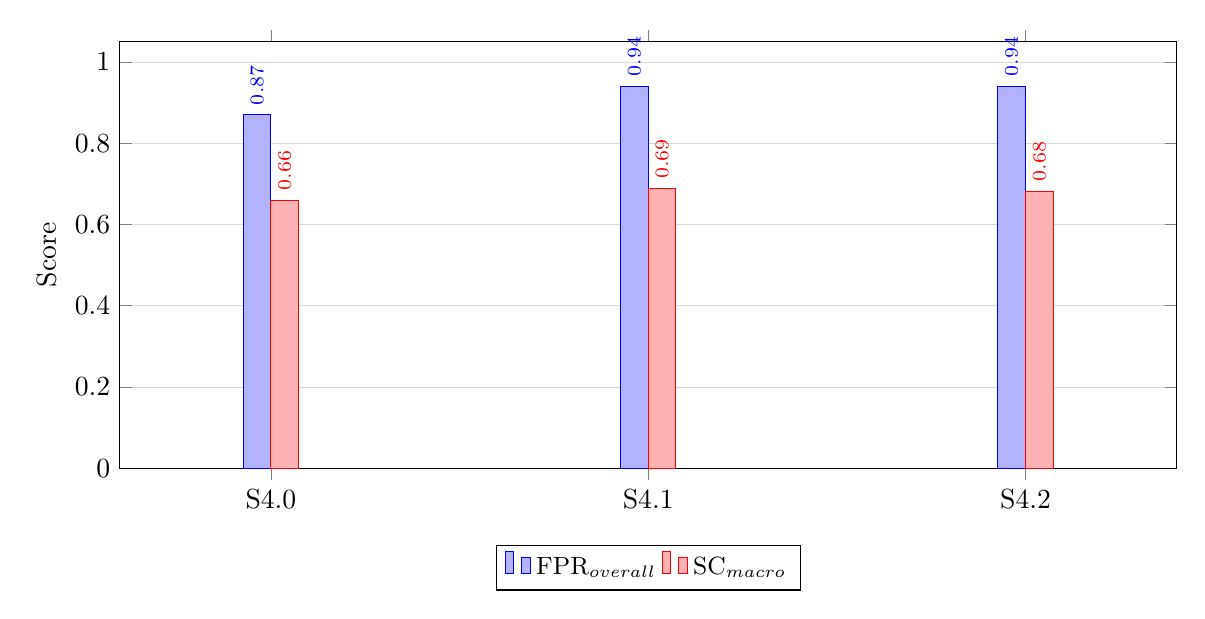
\begin{tikzpicture}
  \begin{axis}[
    width=15cm,
    height=7cm,
    ybar=0pt,
    bar width=10pt,
    ymin=0, ymax=1.05,
    ylabel={Score},
    symbolic x coords={S4.0,S4.1,S4.2},
    xtick=data,
    ymajorgrids=true,
    grid style={line width=0.3pt, draw=gray!30},
    legend style={at={(0.5,-0.18)}, anchor=north, legend columns=2, font=\small},
    enlarge x limits=0.20,
    nodes near coords,
    nodes near coords style={
        font=\scriptsize,
        rotate=90,     % vertical text
        anchor=west,
    }
  ]
    % FPR_overall
    \addplot coordinates {(S4.0,0.870) (S4.1,0.940) (S4.2,0.940)};
    \addlegendentry{$\mathrm{FPR}_{\text{overall}}$}

    % SC_macro
    \addplot coordinates {(S4.0,0.6599) (S4.1,0.6881) (S4.2,0.6815)};
    \addlegendentry{$\mathrm{SC}_{\text{macro}}$}
  \end{axis}
\end{tikzpicture}
\caption{Consistency (S4 variants): schema formatting vs.\ input-aware style.}
\label{fig:s4-consistency}
\end{figure}

